% !TEX root = ../ui-thesis.tex
% !TeX program = xelatex

\chapter{بررسی پیشینه و ادبیات}
\section{ادبیات موضوع}
\subsection{چگونگی کار معماری \lr{RWKV}:}

\lr{RWKV} \cite{RWKV} \cite{peng2024eagle} یک معماری شبکه عصبی است که ترکیبی از مزایای شبکه‌های عصبی بازگشتی \LTRfootnote{Recurrent Neural Networks} \cite{1808.03314} و ترانسفورمرها \LTRfootnote{Transformers} \cite{1706.03762} را به کار می‌گیرد. این معماری برای پردازش کارآمد دنباله‌های داده طراحی شده است، مانند \lr{RNN} ها، اما همچنین از قابلیت‌های پردازش موازی ترانسفورمرها بهره می‌برد. این رویکرد ترکیبی به \lr{RWKV} اجازه می‌دهد تا وابستگی‌های بلندمدت در داده‌ها را حفظ کند، که این مسئله برای \lr{RNNs} سنتی به دلیل مشکلاتی مانند مشکل ناپدید شدن گرادیان چالش‌برانگیز است. در عین حال، از مقیاس‌پذیری و عملکرد ترانسفورمرها، به ویژه در طول آموزش، بهره‌مند می‌شود. به طور کلی، \lr{RWKV} می‌تواند به صورت موازی مانند ترانسفورمرها آموزش ببیند اما در زمان استنتاج به صورت دنباله‌ای عمل کند، که این ویژگی آن را هم کارآمد و هم قدرتمند برای وظایف مختلف پردازش زبان طبیعی می‌سازد.

\subsubsection{\lr{RWKV} در مقایسه با \lr{transformer}}
در مورد آموزش یک مدل زبانی برای تولید موسیقی لو-فای، ما تصمیم گرفتیم از معماری \lr{RWKV} به جای معماری ترانسفورمر استفاده کنیم. یکی از دلایل اصلی این انتخاب این است که \lr{RWKV} برای کارایی بیشتر و اجرای آسان‌تر روی \lr{CPU} طراحی شده است که برای پروژه ما مفید است.

به طور خاص، معماری \lr{RWKV} به صورت خطی و ترتیبی است که زمان‌های استنتاج سریع‌تری نسبت به معماری ترانسفورمر فراهم می‌کند. این به این دلیل است که مدل \lr{RWKV} دنباله ورودی را به صورت ترتیبی، یک توکن در هر زمان، پردازش می‌کند، مشابه شبکه‌های عصبی بازگشتی \LTRfootnote{RNNs}. این پردازش ترتیبی به \lr{RWKV} اجازه می‌دهد تا از روابط زمانی در داده‌های ورودی بهره‌برداری کند و زمان‌های استنتاج آن را به طور قابل توجهی سریع‌تر کند.

علاوه بر این، \lr{RWKV} یک مکانیزم توجه \LTRfootnote{Attention mechanism} را در خود جای داده است که به مدل اجازه می‌دهد هنگام تولید توکن بعدی، بر روی بخش‌های خاصی از دنباله ورودی تمرکز کند. این مکانیزم به \lr{RWKV} امکان می‌دهد تا وابستگی‌ها و روابط بلندمدت بین توکن‌ها را به دست آورد، در حالی که همچنان کارایی یک مدل ترتیبی را حفظ می‌کند. مکانیزم توجه در \lr{RWKV} به گونه‌ای طراحی شده است که از نظر محاسباتی کارآمد باشد و از ترکیبی از تبدیل‌های خطی و ضرب نقطه‌ای برای محاسبه وزن‌های توجه استفاده کند.

علاوه بر این، معماری \lr{RWKV} به طور خاص برای پردازش داده‌های جریانی طراحی شده است که یک نیاز کلیدی برای بسیاری از برنامه‌های تولید موسیقی است. \lr{RWKV} داده‌های ورودی را به صورت جریانی پردازش می‌کند، به طوری که هر توکن ورودی به محض ورود پردازش می‌شود، بدون نیاز به بارگذاری کل دنباله ورودی در حافظه. این به \lr{RWKV} اجازه می‌دهد تا دنباله‌های ورودی بزرگ، مانند آهنگ‌ها یا فایل‌های صوتی طولانی، را بدون تمام شدن حافظه مدیریت کند. این قابلیت جریانی همچنین به \lr{RWKV} اجازه می‌دهد تا موسیقی را به صورت بلادرنگ تولید کند، که آن را برای برنامه‌هایی مانند تولید موسیقی زنده یا ابزارهای ترکیب موسیقی مناسب می‌سازد.

علاوه بر این، \lr{RWKV} همچنین زمان‌های آموزش سریع‌تری را فراهم می‌کند، زیرا می‌تواند داده‌های ورودی را به صورت جریانی، یک توکن در هر زمان، پردازش کند، به جای نیاز به بارگذاری کل دنباله ورودی در حافظه به صورت یکجا.

به طور کلی، معماری \lr{RWKV} تعادلی بهتر بین عملکرد، کارایی و سهولت استقرار فراهم می‌کند و آن را به یک انتخاب ایده‌آل برای تولید موسیقی لو-فای تبدیل می‌کند.
\begin{figure}[!htb]
      \centering
      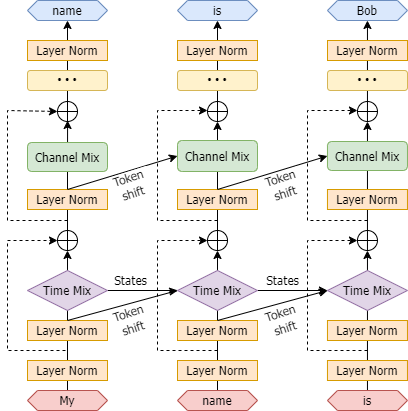
\includegraphics[scale=0.5]{Figures/RWKV-arch.png}
      \caption{معماری \lr{RWKV} برای مدل های زبان
      }
      \label{Fig:RWKV}
\end{figure}

\begin{figure}%
      \centering
      \subfloat[\centering \lr{Residual block}]{{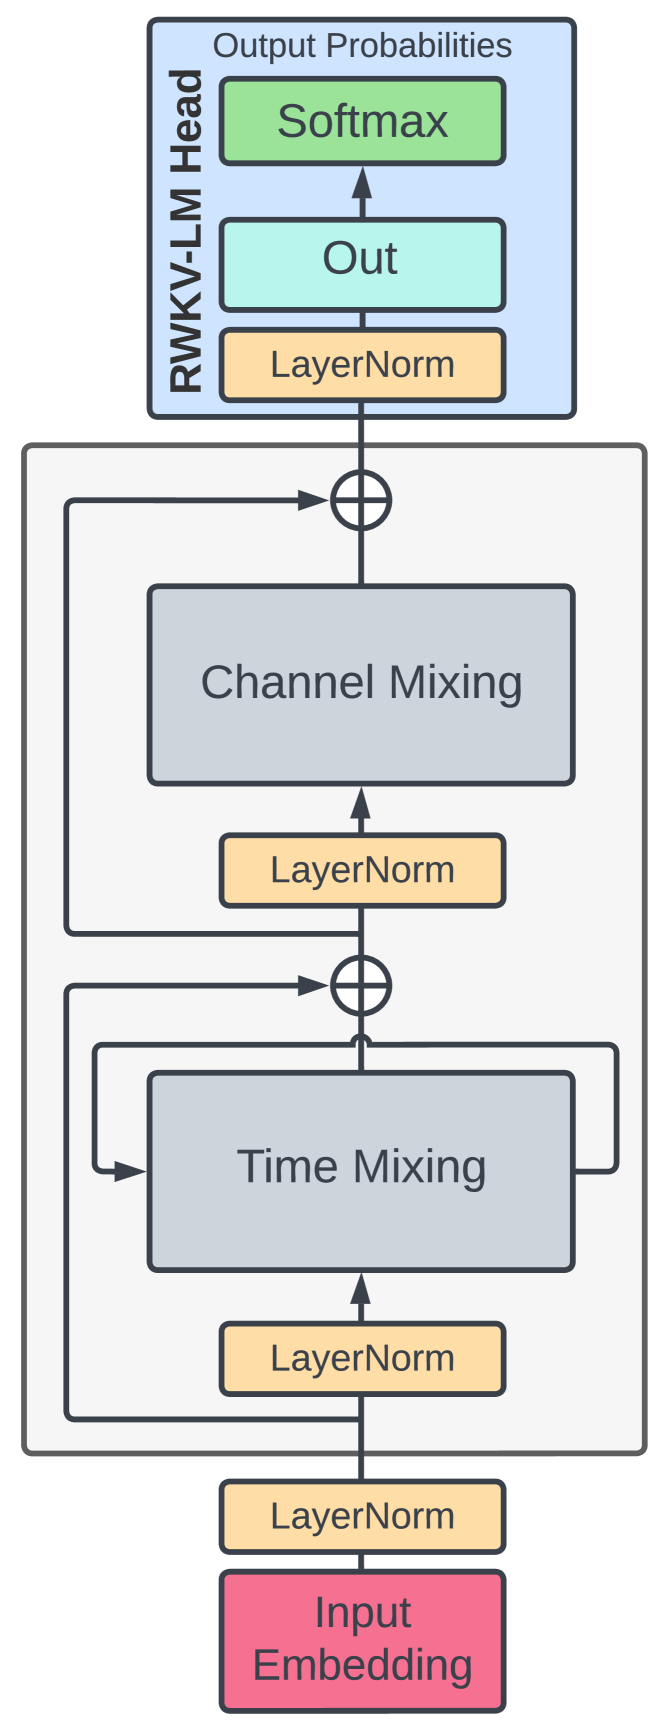
\includegraphics[width=5cm]{Figures/x3.png} }}%
      \qquad
      \subfloat[\centering \lr{Final head of language model}]{{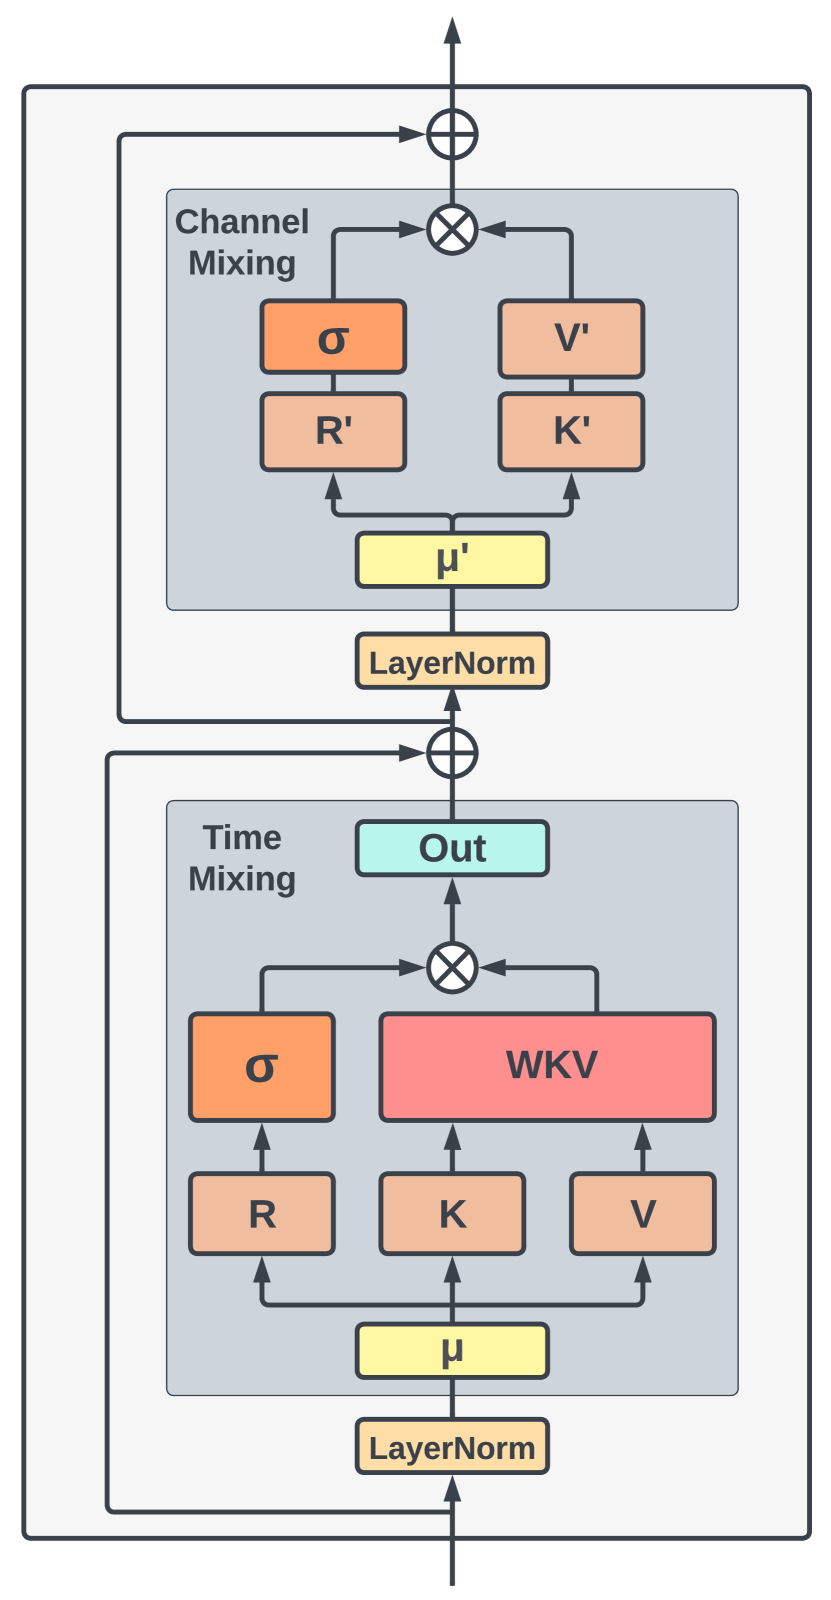
\includegraphics[width=5cm]{Figures/x2.png} }}%
      \caption{عناصر موجود در یک بلوک \lr{RWKV}}
      \label{fig:example}%
\end{figure}

همانطور که در \ref{Fig:RWKV} نشان داده شده است،
مدل با یک لایه \lr{embedding} شروع می‌شود که  . پس از آن، چندین  \lr{residual blocks} مشابه به صورت متوالی قرار گرفته‌اند. این بلوک‌ها در شکل‌های \ref{Fig:RWKVB} نشان داده شده‌اند. پس از آخرین بلوک، یک سر خروجی ساده شامل یک لایه نرمال‌سازی \LTRfootnote{\lr{(LayerNorm)}} و یک پروجکشن خطی برای تولید لاجیت‌ها \LTRfootnote{\lr{(logits)}} جهت پیش‌بینی توکن بعدی و محاسبه‌ی خطای متقاطع \LTRfootnote{\lr{(cross-entropy loss)}} در طول آموزش استفاده می‌شود.

\subsection{فرمت فایل \lr{MIDI}}

فرمت \lr{MIDI} \LTRfootnote{Musical Instrument Digital Interface} \cite{de2017understanding} یک استاندارد فنی برای ارتباط بین ابزارهای موسیقی الکترونیکی، کامپیوترها و دیگر دستگاه‌های مرتبط با موسیقی است. برخلاف فایل‌های صوتی معمولی مانند \lr{MP3} یا \lr{WAV}، فایل‌های \lr{MIDI} حاوی داده‌های صوتی واقعی نیستند. در عوض، آن‌ها شامل اطلاعاتی مانند نت‌های موسیقی، زمان‌بندی، مدت زمان و شدت صدا برای هر نت هستند.

این فرمت به موسیقی‌دانان و تولیدکنندگان موسیقی اجازه می‌دهد تا داده‌های موسیقی را به صورت دیجیتالی ضبط و پخش کنند و به راحتی بین نرم‌افزارها و سخت‌افزارهای مختلف به اشتراک بگذارند. به دلیل اندازه کوچک فایل‌های \lr{MIDI}، انتقال و ذخیره‌سازی آن‌ها بسیار آسان است.

از دیدگاه کامپیوتری، فایل‌های \lr{MIDI} به عنوان مجموعه‌ای از پیام‌های دیجیتالی ذخیره می‌شوند که هر پیام شامل اطلاعاتی درباره نحوه پخش موسیقی است. این پیام‌ها به صورت باینری کدگذاری می‌شوند و شامل سه بخش اصلی هستند:

\begin{enumerate}
      \def\labelenumi{\arabic{enumi}.}
      \item
            \textbf{پیام‌های وضعیت \LTRfootnote{Status Messages}}: این پیام‌ها نوع عملیاتی که
            باید انجام شود را مشخص می‌کنند، مانند نواختن یک نت، تغییر شدت صدا، یا
            تغییر ابزار موسیقی.
      \item
            \textbf{پیام‌های داده \LTRfootnote{Data Messages}}: این پیام‌ها اطلاعات دقیق‌تری
            درباره عملیات مشخص شده در پیام‌های وضعیت ارائه می‌دهند، مانند شماره نت،
            شدت صدا، و مدت زمان.
      \item
            \textbf{زمان‌بندی \LTRfootnote{Timing}}: این بخش زمان دقیق اجرای هر پیام را مشخص
            می‌کند، که به دستگاه‌ها اجازه می‌دهد تا موسیقی را با دقت زمانی بالا پخش
            کنند.
\end{enumerate}

پیام وضعیت: نواختن نت \LTRfootnote{Note On}
پیام داده: شماره نت (مثلاً \lr{C4})، شدت صدا (مثلاً 64)
زمان‌بندی: زمان شروع (مثلاً 500 میلی‌ثانیه پس از شروع)
این پیام‌ها به ترتیب در یک فایل \lr{MIDI} ذخیره می‌شوند و هنگام پخش، دستگاه‌های \lr{MIDI} این پیام‌ها را تفسیر کرده و موسیقی را تولید می‌کنند. این ساختار به کامپیوترها و دستگاه‌های موسیقی اجازه می‌دهد تا به صورت هماهنگ و دقیق موسیقی را پخش کنند.

\begin{figure}[!htb]
      \centering
      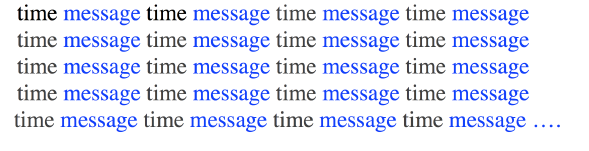
\includegraphics[scale=1]{Figures/Screenshot 2024-08-29 021655.png}
      \caption{ساختار فایل \lr{MIDI}
      }
      \label{Fig:MIDI}
\end{figure}

استفاده از فرمت \lr{MIDI} برای آموزش مدل‌های زبانی نسبت به فرمت \lr{WAV} مزایای
متعددی دارد:

\begin{enumerate}
      \def\labelenumi{\arabic{enumi}.}
      \item
            \textbf{اندازه فایل کوچکتر}: فایل‌های \lr{MIDI} بسیار کوچکتر از فایل‌های \lr{WAV}
            هستند. این امر باعث می‌شود که پردازش و انتقال داده‌ها سریع‌تر و کارآمدتر
            باشد¹.
      \item
            \textbf{داده‌های ساختاریافته}: فایل‌های \lr{MIDI} شامل اطلاعات دقیق و
            ساختاریافته‌ای درباره نت‌های موسیقی، زمان‌بندی، و شدت صدا هستند. این
            داده‌ها به مدل‌های زبانی کمک می‌کنند تا الگوهای موسیقی را بهتر درک کنند و
            پیش‌بینی‌های دقیق‌تری انجام دهند.
      \item
            \textbf{انعطاف‌پذیری بیشتر}: با استفاده از \lr{MIDI}، می‌توان به راحتی
            تغییرات مختلفی در موسیقی اعمال کرد، مانند تغییر تمپو، کلید، و ابزار
            موسیقی. این انعطاف‌پذیری به مدل‌های زبانی کمک می‌کند تا با شرایط مختلف
            سازگار شوند و عملکرد بهتری داشته باشند.
      \item
            \textbf{کاهش نویز}: فایل‌های \lr{WAV} شامل داده‌های صوتی خام هستند که ممکن
            است نویز و اختلالات زیادی داشته باشند. در مقابل، فایل‌های \lr{MIDI} تنها
            شامل داده‌های دیجیتالی هستند که نویز ندارند و این امر باعث می‌شود که
            مدل‌های زبانی با داده‌های تمیزتر و دقیق‌تری آموزش ببینند.
\end{enumerate}

یک مزیت دیگر استفاده از فرمت \lr{MIDI} برای آموزش مدل‌های زبانی این است که موسیقی چندلایه را به خوبی پشتیبانی می‌کند. فایل‌های \lr{MIDI} می‌توانند چندین ترک \LTRfootnote{Track} را به صورت همزمان ذخیره کنند، که هر ترک می‌تواند نمایانگر یک ابزار موسیقی مختلف باشد. این ویژگی به مدل‌های زبانی اجازه می‌دهد تا تعاملات پیچیده بین ابزارهای مختلف را درک کنند و تحلیل کنند که چگونه این ابزارها با هم ترکیب می‌شوند تا یک قطعه موسیقی کامل را تشکیل دهند.

این قابلیت به ویژه برای آموزش مدل‌های زبانی که هدفشان تولید یا تحلیل موسیقی پیچیده است، بسیار مفید است. با داشتن داده‌های چندلایه، مدل‌ها می‌توانند به درک عمیق‌تری از ساختار موسیقی برسند و پیش‌بینی‌های دقیق‌تری انجام دهند.

\section{روشهای پيشين}
\subsection{استفاده از معماری \lr{VAE}}
پروژه \lr{jacbz/Lofi} \cite{Zhang} با استفاده از معماری \lr{VAE} کار مشابهی را انجام می دهد.
استفاده از معماری \lr{RWKV}، معماری که ما در این پروژه استفاده کرده‌ایم، برای ساخت موزیک
لوفای \LTRfootnote{Lo-Fi} مزایای متعددی نسبت به \lr{VAE} \LTRfootnote{Variational Autoencoder} دارد:

\begin{enumerate}
      \def\labelenumi{\arabic{enumi}.}
      \item
            \textbf{حفظ ساختار زمانی}: \lr{RWKV} به دلیل استفاده از مکانیزم‌های بازگشتی،
            قادر است ساختار زمانی و توالی‌های طولانی را بهتر حفظ کند. این ویژگی
            برای موزیک لوفای که اغلب دارای الگوهای تکراری و ریتمیک است، بسیار مهم
            است.
      \item
            \textbf{کیفیت بازسازی بهتر}: \lr{RWKV} به دلیل استفاده از مکانیزم توجه، می‌تواند جزئیات بیشتری از داده‌های ورودی را حفظ کند و بازسازی
            دقیق‌تری ارائه دهد.
      \item
            \textbf{انعطاف‌پذیری بیشتر}: این معماری به دلیل استفاده از مکانیزم‌های
            توجه \LTRfootnote{Attention mechanism} ، می‌تواند به طور دینامیک به بخش‌های مختلف داده توجه کند و این امر
            باعث می‌شود که در تولید موزیک‌های پیچیده‌تر و متنوع‌تر عملکرد بهتری داشته
            باشد.
\end{enumerate}

\subsubsection{محدودیت‌های
     پروژه \lr{jacbz/Lofi}}

\begin{enumerate}
      \def\labelenumi{\arabic{enumi}.}
      \item
            \textbf{محدودیت در اندازه آهنگ}: یکی از محدودیت‌های اصلی \lr{VAE} این است که
            به دلیل استفاده از فضای نهان با ابعاد کمتر، ممکن است در بازسازی
            آهنگ‌های طولانی‌تر دچار مشکل شود. این امر می‌تواند منجر به از دست رفتن
            جزئیات مهم و کاهش کیفیت بازسازی شود⁴.
      \item
            \textbf{کیفیت بازسازی پایین‌تر}: \lr{VAE} به دلیل استفاده از توزیع‌های
            احتمالاتی برای بازسازی داده‌ها، ممکن است در بازسازی جزئیات دقیق دچار
            مشکل شود و کیفیت نهایی موزیک کاهش یابد⁴.
\end{enumerate}
به طور کلی، معماری \lr{RWKV} به دلیل توانایی بهتر در حفظ ساختار زمانی و
جزئیات داده‌ها، برای ساخت موزیک لوفای مناسب‌تر است. از طرف دیگر، \lr{VAE} به
دلیل محدودیت‌های ذاتی خود در بازسازی آهنگ‌های طولانی و پیچیده، ممکن است
کیفیت نهایی موزیک را کاهش دهد.

\subsection{استفاده از معماری \lr{RNN LSTM}}

استفاده از معماری \lr{RWKV} برای ساخت موزیک لوفای مزایای متعددی نسبت به \lr{LSTM} \LTRfootnote{Long Short-Term Memory} دارد. \lr{RWKV} به دلیل استفاده از مکانیزم‌های کلید-مقدار وزنی، قادر است ساختار زمانی و توالی‌های طولانی را بهتر حفظ کند. این ویژگی برای موزیک لوفای که اغلب دارای الگوهای تکراری و ریتمیک است، بسیار مهم است. همچنین، \lr{RWKV} به دلیل استفاده از کلیدها و مقادیر وزنی، می‌تواند جزئیات بیشتری از داده‌های ورودی را حفظ کند و بازسازی دقیق‌تری ارائه دهد. این معماری به دلیل استفاده از مکانیزم‌های توجه \LTRfootnote{Attention mechanism}، می‌تواند به طور دینامیک به بخش‌های مختلف داده توجه کند و این امر باعث می‌شود که در تولید موزیک‌های پیچیده‌تر و متنوع‌تر عملکرد بهتری داشته باشد.

از سوی دیگر، یکی از محدودیت‌های اصلی \lr{LSTM} این است که به دلیل استفاده از حافظه کوتاه مدت، ممکن است در بازسازی آهنگ‌های طولانی‌تر دچار مشکل شود. این امر می‌تواند منجر به از دست رفتن جزئیات مهم و کاهش کیفیت بازسازی شود. همچنین، \lr{LSTM} به دلیل استفاده از توزیع‌های احتمالاتی برای بازسازی داده‌ها، ممکن است در بازسازی جزئیات دقیق دچار مشکل شود و کیفیت نهایی موزیک کاهش یابد.

به طور کلی، معماری \lr{RWKV} به دلیل توانایی بهتر در حفظ ساختار زمانی و جزئیات داده‌ها، برای ساخت موزیک لوفای مناسب‌تر است. از طرف دیگر، \lr{LSTM} به دلیل محدودیت‌های ذاتی خود در بازسازی آهنگ‌های طولانی و پیچیده، ممکن است کیفیت نهایی موزیک را کاهش دهد.
